\subsection{HOMOGENEOUS SPACES AND QUOTIENT GROUPS}

PROPOSITION 11. Let \(\mathbf{X}\) be a Lie group and \(\mathbf{G}\) a Lie subgroup of \(\mathbf{X}\) .

\begin{enumerate}
\def\labelenumi{(\roman{enumi})}
\item
  There exists on the homogeneous set X/G one and only one analytic manifold structure such that the canonical projection \(\pi\) of X onto X/G is a submersion. The law of operation of X on X/G is analytic. For all \(x \in X\) , the kernel of \(\mathrm{T}_{x}(\pi)\) is obtained from \(\mathrm{T}_{e}(\mathrm{G})\) by \(\mathrm{T}_{e}(\gamma(x))\) .
\item
  If \(\mathbf{G}\) is normal in \(\mathbf{X}\) , \(\mathbf{X} / \mathbf{G}\) is a Lie group with its group structure and the manifold structure defined in (i). The mapping \(\pi\) is a Lie group morphism.
\end{enumerate}

By General Topology, Chapter III, § 4, no. 1, Example 1, G operates properly and freely on X by right translation. Hence the first assertion of (i) follows from

Proposition 10 of no. 5. The second follows from the Remark of no. 5. Since \(\pi\) is a submersion, the kernel of \(T_{x}(\pi)\) is the tangent space at \(x\) to

\[
\pi^ {- 1} (\pi (x)) = x \mathrm{G} = \gamma (x) (\mathrm{G})
\]

and hence is obtained from \(T_{e}(G)\) by \(T_{e}(\gamma(x))\) .

Suppose that G is normal. Let \(m\) be the mapping \((x,y)\mapsto xy^{-1}\) of \((\mathrm{X / G})\times (\mathrm{X / G})\) into X/G. Then \((m\circ (\pi \times \pi))(x,y) = \pi (xy^{-1})\) for all \(x,y\) in X. Hence \(m\circ (\pi \times \pi)\) is analytic. As \(\pi \times \pi\) is a surjective submersion, \(m\) is analytic (Differentiable and Analytic Manifolds, R. 5.9.5), whence (ii).

The homogeneous set X/G with the manifold structure defined in (i) is called the quotient (left) Lie homogeneous space of X by G. The (right) Lie homogeneous space G\\backslash X is defined analogously. When G is normal, the Lie group X/G defined in (ii) is called the quotient Lie group of X by G.

PROPOSITION 12. Let X be a Lie group and Y a non-empty analytic manifold with a law of analytic left operation of X on Y. For all \(y \in Y\) , let \(\rho(y)\) be the orbital mapping by y and \(X_{y}\) the stabilizer of y in X. The following conditions are equivalent:

\begin{enumerate}
\def\labelenumi{(\roman{enumi})}
\tightlist
\item
  there exists \(y \in \mathbf{Y}\) such that \(\rho(y)\) is a surjective submersion;
\end{enumerate}

(i') for all \(y \in Y\) , \(\rho(y)\) is a surjective submersion;

\begin{enumerate}
\def\labelenumi{(\roman{enumi})}
\setcounter{enumi}{1}
\tightlist
\item
  there exists \(y \in Y\) such that \(X_y\) is a Lie subgroup of \(X\) and the canonical mapping of \(X / X_y\) into \(Y\) is a manifold isomorphism;
\end{enumerate}

(ii') for all \(y \in Y\) , \(X_y\) is a Lie subgroup of \(X\) and the canonical mapping of \(X / X_y\) into \(Y\) is a manifold isomorphism;

\begin{enumerate}
\def\labelenumi{(\roman{enumi})}
\setcounter{enumi}{2}
\tightlist
\item
  the mapping \((x,y)\mapsto (y,xy)\) of \(\mathbf{X}\times \mathbf{Y}\) into \(\mathbf{Y}\times \mathbf{Y}\) is a surjective submersion.
\end{enumerate}

As the canonical mapping of X onto \(X/X_{y}\) is a submersion, the equivalences (i) \(\Leftrightarrow\) (ii), (i') \(\Leftrightarrow\) (ii') are immediate. (i) \(\Leftrightarrow\) (i') by Proposition 9 of no. 5. The equivalence (i') \(\Leftrightarrow\) (iii) follows from formula (7) of no. 5.

Under the conditions of Proposition 12, Y is called a (left) Lie homogeneous space of X. Right Lie homogeneous spaces of X are defined analogously.

Example. Let \(\mathrm{G}\) be a Lie group. We make \(\mathrm{G} \times \mathrm{G}\) operate on \(\mathrm{G}\) on the left by \((g_1, g_2)x = g_1xg_2^{-1}\) . Let \(\rho\) be the orbital mapping of \(e\) . Then the restrictions of \(\mathrm{T}_{(e,e)}(\rho)\) to \(\mathrm{T}_{(e,e)}(\mathrm{G} \times \{e\}) = \mathrm{T}_e(\mathrm{G}) \times \{0\}\) and to

\[
\mathrm{T} _ {(e, e)} (\{e \} \times \mathrm{G}) = \{0 \} \times \mathrm{T} _ {e} (\mathrm{G})
\]

are isomorphisms of these spaces onto \(\mathrm{T}_{e}(\mathrm{G})\) . Hence \(\mathrm{T}_{(e,e)}(\rho)\) is surjective and \(\mathrm{Ker~T}_{(e,e)}(\rho)\) admits for example the topological supplement \(\mathrm{T}_{e}(\mathrm{G}) \times \{0\}\) in \(\mathrm{T}_{(e,e)}(\mathrm{G} \times \mathrm{G})\) . Thus \(\rho\) is a submersion at \((e,e)\) . Hence G is a left Lie homogeneous space of \(\mathrm{G} \times \mathrm{G}\) .

PROPOSITION 13. Let G be a Lie group, H a normal Lie subgroup of G, X a manifold of class \(\mathbf{C}^r\) and \((g,x)\mapsto gx\) a law of left operation of class \(\mathbf{C}^r\) of G on X. Suppose that conditions (a) and (b) of Proposition 10 hold.

\begin{enumerate}
\def\labelenumi{(\roman{enumi})}
\item
  The law of left operation \((h, x) \mapsto hx\) of H on X satisfies conditions (a) and (b) of Proposition 10 (so that we can consider the quotient manifolds \(\mathbf{X} / \mathbf{G}\) and \(\mathbf{X} / \mathbf{H}\) ).
\item
  The law of left operation of G on X defines on taking quotients a law of left operation of class \(C^{r}\) of G/H on X/H; this law satisfies conditions (a) and (b) of Proposition 10 (so that we can consider the quotient manifold \((\mathrm{X}/\mathrm{H})/(\mathrm{G}/\mathrm{H})\) ).
\item
  The canonical mapping of X onto X/H defines on taking quotients a bijection of X/G onto (X/H)/(G/H). This bijection is an isomorphism of manifolds of class \(\mathbf{C}^r\) .
\end{enumerate}

Clearly H operates freely on X; it operates properly by General Topology, Chapter III, § 4, no. 1, Example 1. The orbital mappings of H on X are immersions since the canonical injection of H into G is an immersion. This proves (i).

The law of left operation of G on X obviously defines, on taking quotients, a law of left operation of G/H on X/H. This law is of class \(C^{r}\) by Differentiable and Analytic Manifolds, R, 5.9.6. Let \(g \in G\) and \(x \in X\) be such that \((\mathrm{Hg})(\mathrm{Hx}) = \mathrm{Hx}\) ; then \(\mathrm{H}(gx) = \mathrm{Hx}\) and hence \(gx \in \mathrm{Hx}\) and \(g \in H\) ; this proves that G/H operates freely on X/H. The mapping \(\theta: (g, x) \mapsto (x, gx)\) of \(G \times X\) into \(X \times X\) is closed; on the other hand, \(\theta(\mathrm{Hg} \times \mathrm{Hx}) = \mathrm{Hx} \times \mathrm{H}(gx)\) ; it follows immediately that the mapping

\[
(\mathrm{Hg}, \mathrm{Hx}) \mapsto (\mathrm{Hx}, \mathrm{H} (g x))
\]

of \((\mathrm{G / H})\times (\mathrm{X / H})\) into \((\mathrm{X / H})\times (\mathrm{X / H})\) is closed; as moreover \(\mathrm{G / H}\) operates freely on \(\mathrm{X / H}\) , Theorem 1 (c) of General Topology, Chapter I, § 10, no. 2 proves that \(\mathrm{G / H}\) operates properly on \(\mathrm{X / H}\) .

Let \(\pi\) be the canonical mapping of X onto X/H, \(\sigma\) the canonical mapping of G onto G/H, \(x\) an element of X and \(y = \pi(x)\) .

\pandocbounded{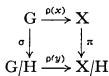
\includegraphics[keepaspectratio]{images/part002_b1d03d5a.jpg}}

Then \(\pi \circ \rho (x) = \rho (y)\circ \sigma\) and hence

\[
\mathrm{T} _ {x} (\pi) \circ \mathrm{T} _ {e} (\rho (x)) = \mathrm{T} _ {e} (\rho (y)) \circ \mathrm{T} _ {e} (\sigma).
\]

Let \(u \in T_{e}(\mathrm{G/H})\) be such that \(T_{e}(\rho(y))u = 0\) . There exists \(v \in T_{e}(\mathrm{G})\) such that \(u = T_{e}(\sigma)v\) . Then \(T_{x}(\pi)(T_{e}(\rho(x))v) = 0\) , hence \(T_{e}(\rho(x))v\) is tangent to Hx (Differentiable and Analytic Manifolds, R, 5.10.5) and therefore is of the form \(T_{e}(\rho(x) | H)v'\) for some \(v' \in T_{e}(\mathrm{H})\) . As \(T_{e}(\rho(x))\) is injective, it follows that \(v = v'\) , whence \(v \in T_{e}(\mathrm{H})\) and therefore \(u = 0\) . Thus \(T_{e}(\rho(y))\) is injective. The image of \(T_{e}(\rho(y))\) is equal to that of \(T_{x}(\pi) \circ T_{e}(\rho(x))\) ; now the image of \(T_{e}(\rho(x))\) admits a topological supplement in \(T_{x}(\mathrm{X})\) and contains the kernel of \(T_{x}(\pi)\) . It is therefore seen that \(\rho(y)\) is an immersion, which completes the proof of (ii).

Assertion (iii) follows from the above and Differentiable and Analytic Manifolds, R, 5.9.7.

COROLLARY. Let G be a Lie group and H and L normal Lie subgroups of G with \(L \subset H\) . Then H/L is a normal Lie subgroup of G/L and the canonical bijection of G/H onto \((G/L)/(H/L)\) is a Lie group isomorphism.

